\section{Introduction}

\subsection{Problem}
\begin{frame}{Problem}{}
  Hvad vil vi?
  \begin{itemize}
  \item Vi vil lave et framework som kan hjælpe ETL programmører med at teste deres systemer
  \end{itemize}
\end{frame}

\begin{frame}{Problem}{}
  Det nuværende marked
  \begin{itemize}
  \item<2-> Table comparisons
    \begin{itemize}
    \item e.g. AnyDBTest
    \item Pro: Folk kan lave assertions omkring stort set alt
    \item Con: Kræver meget kodning, hvor man nemt kan lave fejl
    \end{itemize}
  \item<3-> GUI baseret testing
    \begin{itemize}
    \item e.g. QuerySurge
    \item Pro: Kræver ikke meget kode
    \item Con: GUI baseret og kan hurtigt blive kompleks.
    \end{itemize}
  \end{itemize}
\end{frame}


\begin{frame}{Problem}{}
  Kriterier til vores framework
  \begin{itemize}
  \item<2-> Frameworket skal kunne bruges til automation af tests
    \begin{itemize}
    \item Vi vil gerne understøtte Agile tilgange
    \end{itemize}
  \item<3-> Det skal være kode orienteret
    \begin{itemize}
    \item Samme filosofi som pygrametl
    \end{itemize}
  \item<4-> Frameworket skal mindske det krævede kode som skal skrives for at udføre ens tests
    \begin{itemize}
    \item Mindre test kode leder som udgangspunkt til mindre bugs i ens tests
    \item Mindre test kode er som ugangspunkt hurtigere at skrive
    \end{itemize}
  \end{itemize}
\end{frame}

\subsection{SkiRaff}

\begin{frame}{SkiRaff}{}
  SkiRaff
  \begin{itemize}
  \item<2-> Et framework til at teste ETL programmer
  \item<3-> Man laver assertions om ens populated DW ved hjælp af Predicates
    \begin{itemize}
      \item Disse Predicates modelere typiske ting som man vil teste for og kan tilpasses til ens DW
    \end{itemize}
  \item<4-> Kan lave funktionelle tests på et system niveau
    \begin{itemize}
    \item Pro: Vi tester systemet som en helhed, og kan fange fejl som er skyldet af at flere komponeneter interagere med hinanden
    \item Con: Gør at det er svært at finde ud af præcis hvor fejl opstår
    \end{itemize}
  \item<5-> Funktionalitet til at man kan udskifte data kilder til test data kilder
    \begin{itemize}
    \item Hvis man bruger pygrametl
    \end{itemize}
  \item<6-> Bygget til at kunne samarbejde med pygrametl
    \begin{itemize}
    \item Kan dog sagtens bruges uden
    \end{itemize}
  \item<7-> Kan bruges sammen med PEP249 compatible DBMS'er
  \end{itemize}
\end{frame}

\begin{frame}{SkiRaff}{}
  Overview af frameworkets komponenter
  \begin{figure}
    \centering
    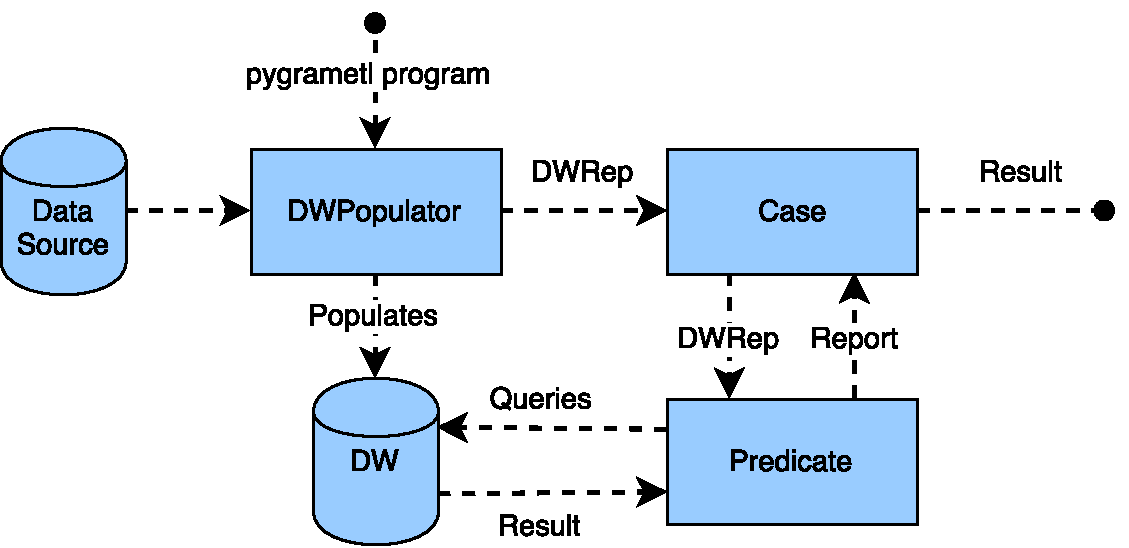
\includegraphics[width=1\textwidth]{figures/overview.pdf}
    \caption{Overview af SkiRaff}
    \label{overview}
  \end{figure}
\end{frame}


\subsection{Demo}

\begin{frame}{Demo}{}
  Demo Af SkiRaff
  \begin{figure}
    \centering
    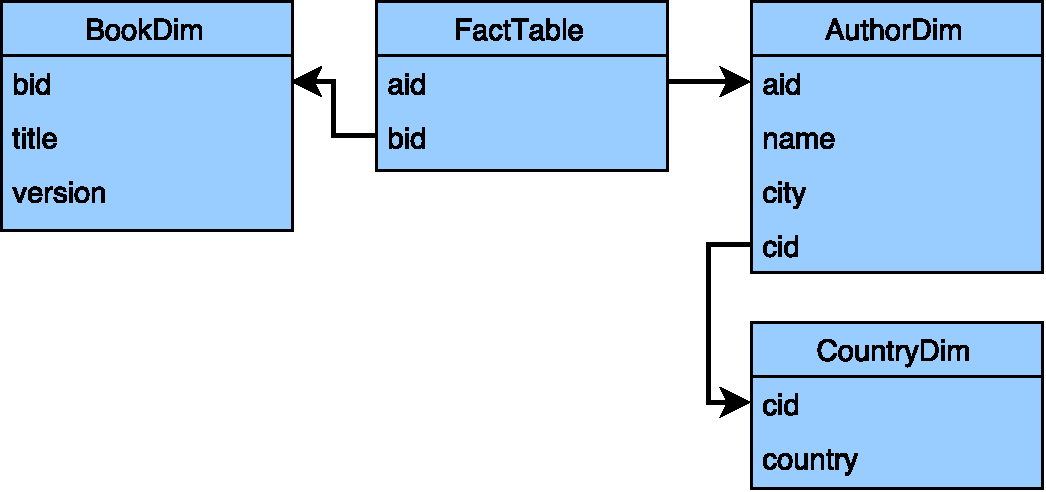
\includegraphics[width=1\textwidth]{figures/example_dw.pdf}
    \caption{DW brugt til demo}
    \label{demodw}
  \end{figure}
\end{frame}
